\chapter{Data}
\label{Da}

This study uses daily finacial data for all the constituents of the Oslo Stock Exchange All-Share Index (OSEAX), obtained from Factset, between January 2010 and September 2017. Stocks that are not continuously listed during the period is excluded. In addition, we have excluded stocks following the criterion employed by Fu \cite{Fu}, which requires that each stock be traded for a minimum of 15 days during each month of the sample period. The number of constituents in the index is 168 before cleaning and <number> after cleaning. This paper is based on the cleaned data. For the constituents of the OSEAX, after data cleaning, we refer to appendix B.

\begin{figure}[h]
    \centering
    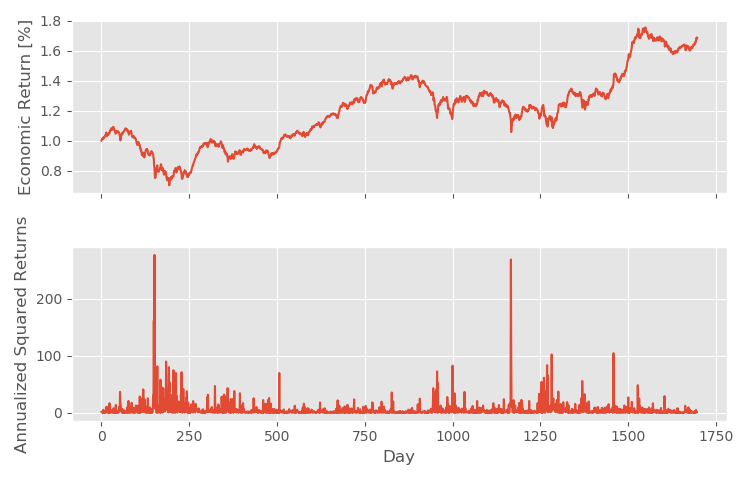
\includegraphics[scale = 0.65]{Plot/MarketReturn.png}
    \caption{Economic Return of the Equally Weighted Market Portfolio}
    \label{Scatter regression}
\end{figure}


\newcolumntype{P}[1]{>{\centering\arraybackslash}p{#1}}
%\begin{landscape}
\begin{longtable}{P{2cm}P{1cm}P{1cm}P{2cm}P{2cm}P{2cm}P{1cm}P{1.5cm}} 
\caption{Descriptive Statistics of the Equally Weighted Market Portfolio}
\label{RegressionIndividualStocks}\\
\hline
\textbf{Observations} & \textbf{Min} & \textbf{Max}&$\boldsymbol{E(r_{economic})}$ &$\boldsymbol{\sigma^2_{economic}}$ &$\boldsymbol{\sigma_{economic}}$ & \textbf{Skew} & \textbf{Kurt} \\
\hline
\endfirsthead
\multicolumn{8}{c}%
{\tablename\ \thetable\ -- \textit{Continued from previous page}} \\
\hline
\textbf{Figure} & \textbf{Observations} & \textbf{Adj. }$\boldsymbol{R^{2}}$ & \textbf{Intercept} & \textbf{P-Value} & \textbf{Beta} & \textbf{P-Value} \\
\hline
\endhead
\hline \multicolumn{8}{r}{\textit{Continued on next page}} \\
\endfoot
\hline
\endlastfoot
\input{Input/DescriptiveStatsTable.txt}
\end{longtable}

%This paper will use continuously compounded returns, $r_c$, defined as: 
%    \begin{align} 
%        e^r_{c,t} = \frac{s_{t}}{s_{t-1}}\\
%        r_c = ln\frac{s_{t}}{s_{t-1}}
%    \end{align}
